\documentclass[../main.tex]{subfiles}
\begin{document}
\subsection{Moto con velocità costante}
\begin{itemize}
    \item $d = V_0t$
    \item $x = d\cos \alpha \phantom{-}$ e $\phantom{-}y = d\sin \alpha$
    \item $V_{0x} = V_0 \cos \alpha \phantom{-}$ e $\phantom{-} V_{0y} = V_0 \sin \alpha$
    \item $x = x_0 + V_{0x}t \phantom{-}$ e $\phantom{-} y = y_0 + V_{0y}t$
\end{itemize}

\begin{center}
    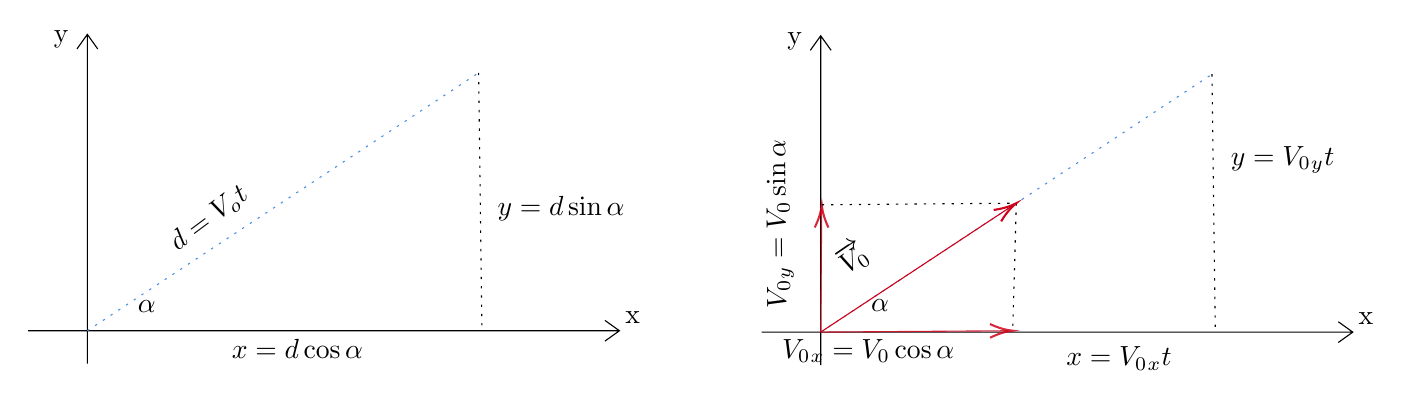
\begin{tikzpicture}[x=0.75pt,y=0.75pt,yscale=-1,xscale=1]
        \draw  (12.67,208.35) -- (297.51,208.35)(41.15,65.58) -- (41.15,224.21) (290.51,203.35) -- (297.51,208.35) -- (290.51,213.35) (36.15,72.58) -- (41.15,65.58) -- (46.15,72.58)  ;
        %Straight Lines [id:da3733649010101341] 
        \draw [color={rgb, 255:red, 74; green, 144; blue, 226 }  ,draw opacity=1 ] [dash pattern={on 0.84pt off 2.51pt}]  (41.15,208.35) -- (229.65,84.1) ;
        %Straight Lines [id:da8110263401690938] 
        \draw  [dash pattern={on 0.84pt off 2.51pt}]  (229.65,84.1) -- (231.29,208.47) ;
        %Shape: Axis 2D [id:dp9174087368813065] 
        \draw  (366,209.01) -- (650.84,209.01)(394.48,66.24) -- (394.48,224.88) (643.84,204.01) -- (650.84,209.01) -- (643.84,214.01) (389.48,73.24) -- (394.48,66.24) -- (399.48,73.24)  ;
        %Straight Lines [id:da11766082667505762] 
        \draw [color={rgb, 255:red, 74; green, 144; blue, 226 }  ,draw opacity=1 ] [dash pattern={on 0.84pt off 2.51pt}]  (394.48,209.01) -- (582.98,84.77) ;
        %Straight Lines [id:da3334719016736133] 
        \draw  [dash pattern={on 0.84pt off 2.51pt}]  (582.98,84.77) -- (584.62,209.13) ;
        %Straight Lines [id:da20336215134398827] 
        \draw [color={rgb, 255:red, 208; green, 2; blue, 27 }  ,draw opacity=0.85 ]   (394.48,209.01) -- (394.98,149.67) ;
        \draw [shift={(395,147.67)}, rotate = 90.48] [color={rgb, 255:red, 208; green, 2; blue, 27 }  ,draw opacity=0.85 ][line width=0.75]    (10.93,-3.29) .. controls (6.95,-1.4) and (3.31,-0.3) .. (0,0) .. controls (3.31,0.3) and (6.95,1.4) .. (10.93,3.29)   ;
        %Straight Lines [id:da4951575276164567] 
        \draw [color={rgb, 255:red, 208; green, 2; blue, 27 }  ,draw opacity=0.85 ]   (394.48,209.01) -- (485,208.35) ;
        \draw [shift={(487,208.33)}, rotate = 179.58] [color={rgb, 255:red, 208; green, 2; blue, 27 }  ,draw opacity=0.85 ][line width=0.75]    (10.93,-3.29) .. controls (6.95,-1.4) and (3.31,-0.3) .. (0,0) .. controls (3.31,0.3) and (6.95,1.4) .. (10.93,3.29)   ;
        %Straight Lines [id:da038864238023705644] 
        \draw  [dash pattern={on 0.84pt off 2.51pt}]  (395,147.67) -- (488.73,146.89) ;
        %Straight Lines [id:da5178148052347968] 
        \draw  [dash pattern={on 0.84pt off 2.51pt}]  (488.73,146.89) -- (487,208.33) ;
        %Straight Lines [id:da25487761251251817] 
        \draw [color={rgb, 255:red, 208; green, 2; blue, 27 }  ,draw opacity=1 ]   (394.48,209.01) -- (487.06,147.99) ;
        \draw [shift={(488.73,146.89)}, rotate = 146.61] [color={rgb, 255:red, 208; green, 2; blue, 27 }  ,draw opacity=1 ][line width=0.75]    (10.93,-3.29) .. controls (6.95,-1.4) and (3.31,-0.3) .. (0,0) .. controls (3.31,0.3) and (6.95,1.4) .. (10.93,3.29)   ;
        
        % Text Node
        \draw (299.07,197.82) node [anchor=north west][inner sep=0.75pt]   [align=left] {x};
        % Text Node
        \draw (23.81,62.6) node [anchor=north west][inner sep=0.75pt]   [align=left] {y};
        % Text Node
        \draw (64.22,192.5) node [anchor=north west][inner sep=0.75pt]    {$\alpha $};
        % Text Node
        \draw (77.32,162.49) node [anchor=north west][inner sep=0.75pt]  [rotate=-323.28]  {$d=V_{o} t$};
        % Text Node
        \draw (237.55,142.23) node [anchor=north west][inner sep=0.75pt]    {$y=d\sin \alpha $};
        % Text Node
        \draw (109.48,211.03) node [anchor=north west][inner sep=0.75pt]    {$x=d\cos \alpha $};
        % Text Node
        \draw (652.41,198.49) node [anchor=north west][inner sep=0.75pt]   [align=left] {x};
        % Text Node
        \draw (377.14,63.27) node [anchor=north west][inner sep=0.75pt]   [align=left] {y};
        % Text Node
        \draw (417.55,191.84) node [anchor=north west][inner sep=0.75pt]    {$\alpha $};
        % Text Node
        \draw (590.89,118.23) node [anchor=north west][inner sep=0.75pt]    {$y=V_{0}{}_{y} t$};
        % Text Node
        \draw (398.22,170.64) node [anchor=north west][inner sep=0.75pt]  [rotate=-325.46]  {$\overrightarrow{V_{0}}$};
        % Text Node
        \draw (367.47,198.75) node [anchor=north west][inner sep=0.75pt]  [rotate=-269.68]  {$V_{0}{}_{y} =V_{0}\sin \alpha $};
        % Text Node
        \draw (511.55,214.89) node [anchor=north west][inner sep=0.75pt]    {$x=V_{0}{}_{x} t$};
        % Text Node
        \draw (374.61,211.26) node [anchor=north west][inner sep=0.75pt]  [rotate=-0.01]  {$V_{0}{}_{x} =V_{0}\cos \alpha $};
    \end{tikzpicture}         
\end{center}

\vspace{1cm}
\subsection{Moto con accellerazione costante}
\begin{itemize}
    \item Posizione in funzione del tempo
    \begin{itemize}
        \item $x(t) = x_0 + V_{0x}t + \frac{1}{2}a_xt^2$
        \item $y(t) = y_0 + V_{0y}t + \frac{1}{2}a_yt^2$
    \end{itemize}
    \item Velocità in funzione del tempo
    \begin{itemize}
        \item $V_x(t) = V_{0x} + a_xt$
        \item $V_y(t) = V_{0y} + a_yt$
    \end{itemize}
    \item Velocità in funzione della Posizione
    \begin{itemize}
        \item $V_x^2 = V_{0x}^2 + 2a_x\Delta x$
        \item $V_y^2 = V_{0y}^2 + 2a_y\Delta y$
    \end{itemize}
\end{itemize}

\vspace{1cm}
\subsection{Moto parabolico}
\begin{itemize}
    \item La resistenza dell'aria \underline{non} viene considerata
    \item L'accellerazione di gravità è costante, verso il basso 
    \begin{itemize}
        \item $\vec{g} = \begin{bmatrix}
            0 \\
            \pm 9.81
        \end{bmatrix}\frac{m}{s^2}$
        \item $g = \pm 9.81\frac{m}{s^2}$
    \end{itemize}
    \item La rotazione della terra viene ignorata
\end{itemize}

\pagebreak
Visto che la componente di accellerazione sull'asse $x$ è nulla, possiamo aggiornare le formule precedenti e ottenere
\begin{itemize}
    \item Posizione in funzione del tempo
    \begin{itemize}
        \item $x(t) = x_0 + V_{0x}t$
        \item $y(t) = y_0 + V_{0y}t - \frac{1}{2}gt^2$
    \end{itemize}
    \item Velocità in funzione del tempo
    \begin{itemize}
        \item $V_x(t) = V_{0x}$
        \item $V_y(t) = V_{0y} - gt$
    \end{itemize}
    \item Velocità in funzione della Posizione
    \begin{itemize}
        \item $V_x^2 = V_{0x}^2$
        \item $V_y^2 = V_{0y}^2 - 2g\Delta y$
    \end{itemize}
\end{itemize}
\textbf{Nota:} La velocità sull'asse $x$ ($V_x$) è costante perchè non c'è accellerazione orizzontale.

\textbf{Nota:} Nelle formule il verso positivo dell'asse $y$ è in alto e si utilizza $a_y = -9.81\frac{m}{s^2} = -g$.

\vspace{1cm}
\subsection{Lancio ad angolo zero (orizzontale)}
Solitamente
\begin{itemize}
    \item $x_0 = 0$
    \item $y_0 = h$
    \item $\alpha = 0$
\end{itemize}

Quindi
\begin{itemize}
    \item $V_{0x} = V_0 \cos 0^\circ = V_0$
    \item $V_{0y} = V_0 \sin  0^\circ = 0$
\end{itemize}

Sostituendo questi valori nelle equazioni del moto troviamo
\begin{itemize}
    \item Posizione in funzione del tempo
    \begin{itemize}
        \item $x(t) = V_{0}t$
        \item $y(t) = h - \frac{1}{2}gt^2$
    \end{itemize}
    \item Velocità in funzione del tempo
    \begin{itemize}
        \item $V_x(t) = V_{0}$
        \item $V_y(t) = - gt$
    \end{itemize}
    \item Velocità in funzione della Posizione
    \begin{itemize}
        \item $V_x^2 = V_{0}^2$
        \item $V_y^2 = - 2g\Delta y$
    \end{itemize}
\end{itemize}

\subsubsection{Altre formule}
\begin{itemize}
    \item Traiettoria (funzione) \begin{align*}
        t(x) =& \frac{x}{V_0} = \sqrt{\frac{2h}{g}}\\
        y =& h - \frac{g}{2V_0^2}x^2
    \end{align*} 
    \item Punto di atterraggio \begin{align*}
        x = V_0 \sqrt{\frac{2h}{g}}
    \end{align*}
\end{itemize}

\vspace{1cm}
\subsection{Lancio ad angolo qualsiasi}
Considerando $x_0 = y_0 = 0$ sappiamo che
\begin{itemize}
    \item Posizione in funzione del tempo
    \begin{itemize}
        \item $x(t) = (V_{0}\cos \alpha) t$
        \item $y(t) = (V_0\sin\alpha)t - \frac{1}{2}gt^2$
    \end{itemize}
    \item Velocità in funzione del tempo
    \begin{itemize}
        \item $V_x(t) = V_{0}\cos\alpha$
        \item $V_y(t) = V_0\sin\alpha- gt$
    \end{itemize}
    \item Velocità in funzione della Posizione
    \begin{itemize}
        \item $V_x^2 = V_{0}^2 \cos^2\alpha$
        \item $V_y^2 =V_0^2\sin^2\alpha - 2g\Delta y$
    \end{itemize}
\end{itemize}

\subsubsection{Proprietà di simmetria della parabola}
Le seguenti considerazioni valgono solo se la parabola è simmetrica
\begin{itemize}
    \item Gittata (o Range, $R$)
    \begin{itemize}
        \item Determiniamo l'istante in cui il proiettile atterra, ponendo $y=0$ nell'equazione \begin{align*}
            y =& \underbrace{x^2(-\frac{g}{2V_0^2\cos^2\alpha}) }_{a<0} + x \underbrace{\tan\alpha }_{b} \phantom{--} c = 0 \\
            y =& (V_0 \sin\alpha)t-\frac{1}{2}gt^2
        \end{align*}
        \item Sostituiamo il tempo trovato nell'equazione del moto in direzione $x$ \begin{align*}
            x = \frac{2V_0^2}{g}\sin\alpha\cos\alpha
        \end{align*}
        che equivale a \begin{align*}
            R = \frac{V_0^2}{g}\sin 2 \alpha
        \end{align*}
    \end{itemize}
    \item Tempo di volo in funzione di velocità iniziale e angolo \begin{align*}
        t = \frac{2V_0}{g}\sin\alpha
    \end{align*}
    \item Altezza massima \begin{align*}
        h_{max} =& \frac{1}{2}R \\
        h_{max} =& \frac{V_0^2\sin^2 \alpha}{2g}
    \end{align*}
\end{itemize}




\end{document}